% !TeX spellcheck = en_B
% !TeX encoding = UTF-8 %%%These comments just make you look like you know what you're doing
\documentclass[8pt]{beamer}  %%% Specifies the class, with 8pt font size

\usepackage[utf8]{inputenc}

\usetheme[block=fill,numbering=fraction,sectionpage=none,background=light]{metropolis}

\usepackage[english]{babel}
\usepackage{csquotes}       
\usepackage[T1]{fontenc}        
\usepackage{booktabs}
\usepackage{pgfgantt}
\usepackage{pifont}
\usepackage{adfbullets}
\usepackage{enumitem}
\usepackage{tikz}
\usepackage{lipsum}
\usepackage{amssymb}
\usepackage{amsfonts}
\usepackage{mathrsfs}
\usepackage{adjustbox}
\usepackage{varioref}
\usepackage{probsoln}
\usepackage{attachfile2}
\usepackage{pgfplots}
\pgfplotsset{compat=newest}
\graphicspath{{Graphics/}}
\usepackage{multirow,array}
\usepackage{colortbl}
\definecolor{aa}{RGB}{255, 124, 0}
\definecolor{cc}{RGB}{230, 230, 230}    
\usebackgroundtemplate{%
    \tikz[overlay,remember picture]{
        \node[scale=0.3,opacity=0.08,xshift=-8cm,yshift=+26.7cm] at (current page.south east){
            
\includegraphics{assets/img/marchio_unitrento_colore_it_202002.eps}
        }
    }
}

%% Indispensables

\usepackage{amsmath}
\usepackage{graphicx}

\usepackage{booktabs}
\newcommand{\ra}[1]{\renewcommand{\arraystretch}{#1}}

\usepackage{tabularx}

%% bibliography
\usepackage[backend=bibtex,style=verbose-trad2]{biblatex}
\bibliography{bibliography.bib}

%% listings
\usepackage{listings}
\usepackage{xcolor}

\colorlet{punct}{red!60!black}
\definecolor{background}{HTML}{EEEEEE}
\definecolor{delim}{RGB}{20,105,176}
\colorlet{field}{magenta!60!black}

\lstdefinelanguage{json}{
    basicstyle=\small\tt,
    numberstyle=\scriptsize,
    showstringspaces=false,
    breaklines=true,
    frame=none,
    literate=
      {,}{{{\color{punct}{,}}}}{1}
      {\{}{{{\color{delim}{\{}}}}{1}
      {\}}{{{\color{delim}{\}}}}}{1}
      {[}{{{\color{delim}{[}}}}{1}
      {]}{{{\color{delim}{]}}}}{1},
    string=[s]{"}{"},
    stringstyle=\color{field},
    comment=[l]{:},
    commentstyle=\color{black},
}

\usepackage{comment}
\usepackage{varwidth}

\newcommand{\mat}[4]{\left(\begin{array}{cc} #1 & #2 \\ #3 & #4 \\ \end{array}\right)}
\newcommand{\Q}{\mathbb{Q}}
\newcommand{\R}{\mathbb{R}}
\newcommand{\Z}{\mathbb{Z}}
\newcommand{\sol}[2][+]{
	\tikz[baseline]{\node[color=aa,fill=cc,rectangle,draw,anchor=base] {  {\onslide<#1->{#2}}  };}
}

\usetikzlibrary{positioning}
\usetikzlibrary{tikzmark}
\usetikzlibrary{shadings}
\usetikzlibrary{through}

\def\height{0.8cm}
\def\width{1.2cm}
\newcommand{\keynode}[6]{\node[minimum height=\height,minimum width=\width,draw,rectangle,color=aa,fill=cc] (#3) at (#1,#2) {};
	\node[rectangle,minimum height=\height/2,minimum width=\width,above,color=aa] at (#3) {#3};
	\node[draw,rectangle,minimum height=\height/2,minimum width=\width/3,below,color=aa,fill=cc,inner sep =0cm] at (#3) {\footnotesize#4};
	\node[draw,rectangle,minimum height=\height/2,minimum width=\width/3,below,xshift=\height/2,color=aa,fill=cc,inner sep=0cm] at (#3) {\footnotesize#5};
	\node[draw,rectangle,minimum height=\height/2,minimum width=\width/3,below,xshift=-\height/2,color=aa,fill=cc,inner sep=0cm] at (#3) {\footnotesize#6}; }

\newenvironment{gantt}[3]{\begin{ganttchart}[#1,bar height=.6,bar top shift=.2,title/.style=  {draw=none},y unit chart=0.6cm,y unit title = 0.6cm,include title in canvas=false,group/.append style={draw=black,dashed},bar/.append style={fill=aa},inline,hgrid=true,Float1/.style={bar/.append style={fill=none,dashed},bar height=.8,bar top shift=0.1}]{#2}{#3}}{\end{ganttchart}}

\newenvironment{nicetable}[1]{\setlength\arrayrulewidth{0.5mm}
			\arrayrulecolor{white}
			\begin{tabular}{#1}}{\end{tabular}}
		
\setlist[itemize,1]{label={\color{aa}\huge\adfbullet{36}}}
\setlist[itemize, 2]{label={\color{aa}\large\adfbullet{36}}}

\newcommand\reshist{}
\def\reshist(#1)#2(#3)#4(#5)%
{\draw (axis cs:#1) rectangle (axis cs:#3) node [midway] {#5};}

\usepackage[
    % hidelinks,
    % colorlinks=true,
]{hyperref} % importare per ultimo

\hypersetup{
    colorlinks = true,
    linkbordercolor = {white}, % rettangoli attorno ai link
    linkcolor = {},     % toc. {} significa nero
    urlcolor = {teal},  % link
    citecolor = {teal}, % bibliografia
}

\usepackage[capitalize, nameinlink, noabbrev]{cleveref} %%%adds the general preamble

%%%Title and subtitle
\title{Studying the emotional impact of the Covid-19 pandemic using social media}
\subtitle{Bachelor Degree Thesis Presentation, \textattachfile{Template.tex}{(TeX)}} %%%This embeds the tikz source code into the resulting pdf...
\author{Simone Alghisi}
\institute{Università degli Studi di Trento}
\date[\today]{\today}

\begin{document}

\frame{\titlepage} %%%Makes titlepage

\setcounter{tocdepth}{1}

\begin{frame}
    \frametitle{Contents}
    \tableofcontents
\end{frame}

\setlength{\abovedisplayskip}{0pt}
\setlength{\belowdisplayskip}{0pt}
\setlength{\abovedisplayshortskip}{0pt}
\setlength{\belowdisplayshortskip}{0pt}  %%%Compresses math

\section{Project description}
\begin{frame}{Introduction to the problem}
The COVID-19 pandemic is having a huge impact on our lives, that goes beyond the direct effects of the virus. Besides the fear of infection, lockdown measures adopted by many countries are limiting the possibility to move, work, have contact with others, and are creating a situation of economic crisis and generalized uncertainty about the future. The psychological effects of this unprecedented situation need to be studied.

The project consisted in an \textbf{analysis of emotions as emerging from Twitter messages} during the pandemic.

\textbf{Lexicon-based sentiment analysis tools} have been employed to characterize emotions associated with content on a large scale. This could allow us to contrast the emotional reaction with the evolution of contagions and deaths, and
with the different lockdown and de-escalation stages, in different areas.

\end{frame}

\section{Dataset and tweets preprocessing}

\begin{frame}{Dataset description and stats}

	The tweets to analyze were retrieved from \textbf{echen102/COVID-19-TweetIDs} GitHub repository\autocite{chen2020tracking} and relate to the period \textbf{from January 2020 to March 2021}. 
	
	Below, some general statistics
	
	\begin{table}[h]
        \centering
        \begin{tabularx}{\textwidth}{lXr}
            Number of files & & \textbf{10 402}
            \\ \lightrule
            Number of identified languages & & \textbf{65}
            \\ \lightrule
            Number of tweets & & \textbf{1 055 843 481}
            \\ \lightrule
            Number of unique tweets (no retweets) & & \textbf{323 504 667}
            \\ \lightrule
            Dataset compressed size & & \textbf{865GB}
            \\ \lightrule
            Dataset estimated uncompressed size & & \textbf{6.252TB}
        \end{tabularx}
    \end{table}

\end{frame}

\begin{frame}{Languages with the most tweets}
    
    % TODO substitute it with real data
	\begin{figure}
	    \centering
	    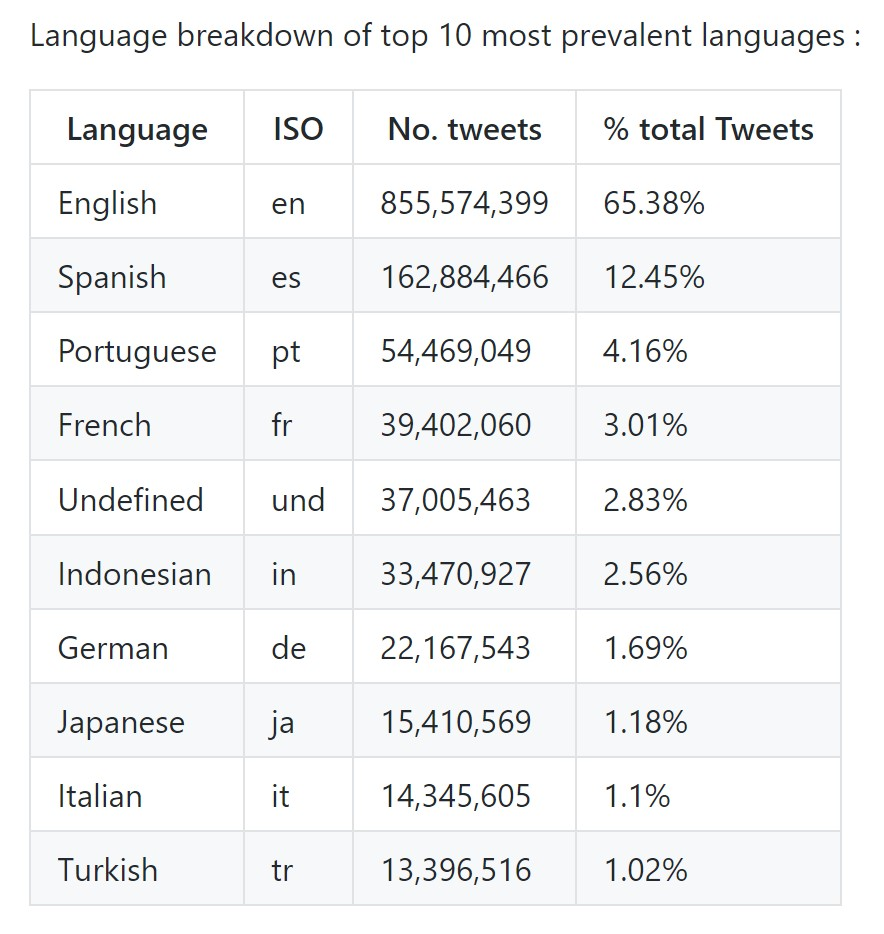
\includegraphics[scale=.5]{assets/img/dataset_most_prevalent_languages.jpg}
	\end{figure}

\end{frame}

\begin{frame}[fragile]{Tweet Structure}

	We retrieved tweets given their id thanks to Twarc and we kept the most relevant information.
	
	\begin{block}{Final JSON object}
    	\begin{lstlisting}[language=json]
{
  "id": 1307025659294674945,
  "full_text": "Here's an article that highlights the updates...",
  "lang": "en",
  "created_at": "Fri Sep 18 18:36:15 +0000 2020",
  "retweet_count": 11,
  "favorite_count": 70,
  "user": {
    "id": 2244994945,
    "id_str": "2244994945",
    "screen_name": "TwitterDev",
    "name": "Twitter Dev",
    "description": "The voice of the #TwitterDev team and your official...",
    "location": "127.0.0.1",
    "followers_count": 513958,
    "statuses_count": 3635,
    "default_profile_image": false,
    "profile_image_url_https": "https:\/\/pbs.twimg.com\/profile_images\/1283786620521652229\/lEODkLTh_normal.jpg"
  }
}
        \end{lstlisting}
	\end{block}
	
\end{frame}

\begin{frame}{Partitioning}

	To access directly to a specific category of tweets (e.g. the tweets written in English on the 3rd of June 2020), we grouped them 
	
	\begin{itemize}
	    \item first according to the \textbf{language}, using the \texttt{lang} field from Twitter
	    \item secondly by \textbf{year-month}
	    \item and finally by \textbf{day}
	\end{itemize}
	
    Later on, we decided to \textbf{aggregate them in weekly batches} for better data visualization and to average the results.

\end{frame}

\section{Sentiment analysis over time - by language}

\begin{frame}{Lexicon}

	We used the NRC Word-Emotion Association Lexicon (aka EmoLex) \autocite{ncrwebsite} for sentiment analysis. EmoLex consists of \textit{" \ldots a list of English words and their associations with \textbf{eight basic emotions} (anger, fear, anticipation, trust, surprise, sadness, joy, and disgust) and \textbf{two sentiments} (negative and positive)."}
	
	\begin{figure}
	    \centering
	    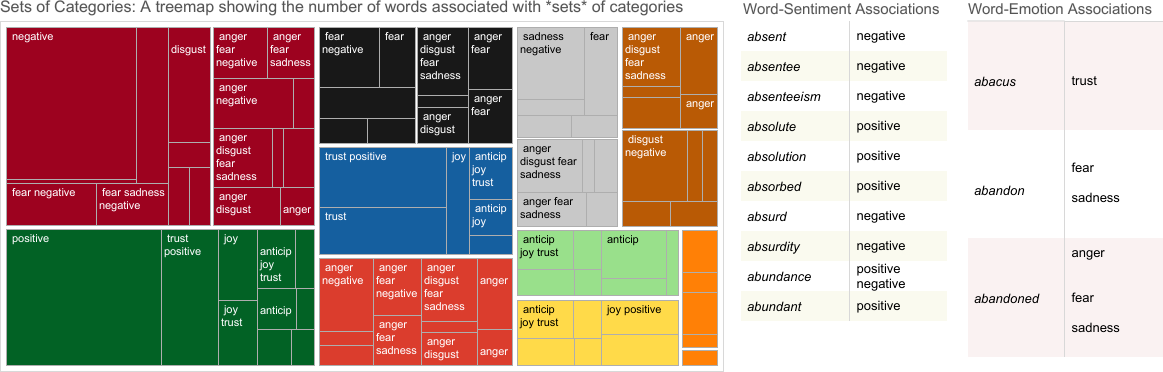
\includegraphics[scale=0.26]{assets/img/NRC Emotion Lexicon.png}
	\end{figure}
	
	We have chosen this lexicon because it \textbf{has been translated in over one hundred languages}.

\end{frame}

\begin{frame}{Languages considered}
    
	We considered \textbf{Catalan, English, Italian} and \textbf{Spanish tweets} for further analysis. This helped to focus on a even more restricted set of data, in particular:
	
	\begin{table}[h]
        \centering
        \begin{tabularx}{\textwidth}{Xrr}
            language & tweets number & tweets percentage \\
            \midrule
                Catalan & 1 377 225 & 0.4\%
                \\ \lightrule
                English & 195 645 826 & 60.4\%
                \\ \lightrule
                Italian & 5 256 748 & 1.6\%
                \\ \lightrule
                Spanish & 35 533 886 & 10.9\%
        \end{tabularx}
        \caption{Number of tweets for a specific language}
        \label{tab:lang_dim}
    \end{table}
	
\end{frame}

\begin{frame}{Methodology}

    However, our statistics could end up biased because of \textbf{particularly active} (or emotional) \textbf{users}.
    
    Given that, we decided to follow one of the approaches discussed by Aiello et al.\autocite{aiello2020epidemic}, in particular we have considered
	
	\begin{itemize}
	    \item \textbf{emotions in a binary way} (e.g. whether in a given week the user expressed joy or not)
	    \item \textbf{users over tweets} (e.g. the number of unique users, instead of tweets, that expressed joy in a week)
	\end{itemize}
	
	\begin{definition}
	    Given \(U_e(t)\), the number of distinct users that expressed emotion \(e\) at time \(t\) in a tweet, and \(U(t)\), the number of distinct users that tweeted at time \(t\),
	    
	    \[f_e(t) = \frac{U_e(t)}{U(t)}\]
	    
	    is the proportion of users that expressed emotion \(e\) at time \(t\).
	\end{definition}

\end{frame}

\subsection{Results per week}
\begin{frame}{Italian tweets per week}
	
	The graphics below shows the proportion of tweets that express a particular emotion (color) w.r.t. the total number of tweets in a week. The dashed grey line indicates the total volume of tweets normalized w.r.t. the maximum value observed in the period Jan 2020-Apr 2021.
	
	\begin{figure}[h]
    	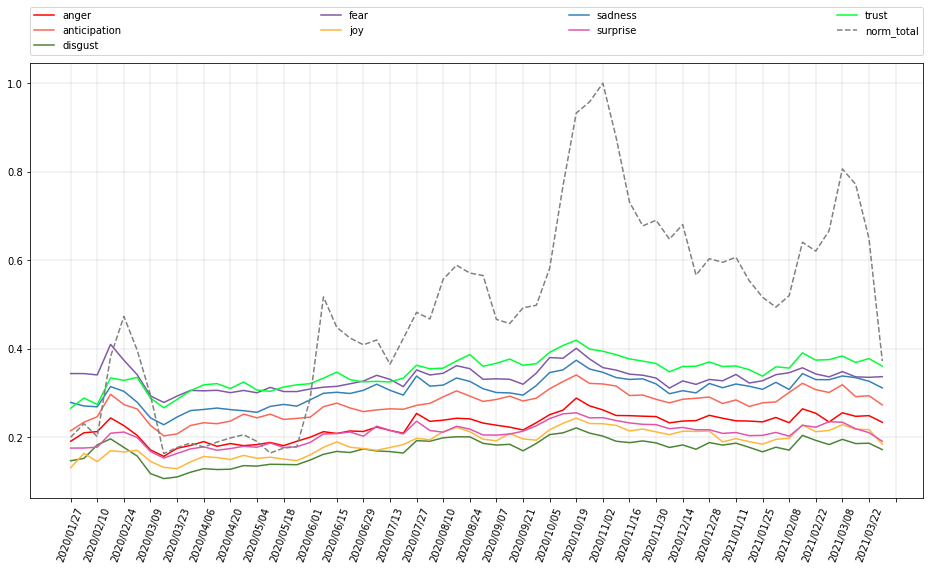
\includegraphics[scale=.29]{assets/img/it_emotions.png}
    	\caption{Emotions expressed in Italian tweets per week.}
    	\label{fig:it_emotion_weekly}
    \end{figure}

\end{frame}


\begin{frame}{Italian tweets per week (subplot)}
	
	The following graphics are just a variation from the one showed before, in order to have a cleaner visualization of the course of a single emotion. 
	
	\begin{figure}[h]
    	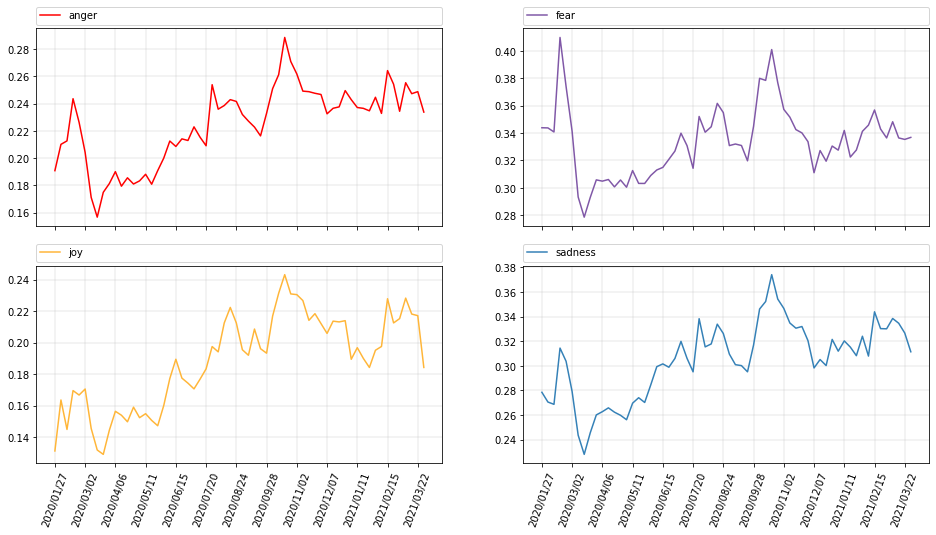
\includegraphics[scale=.3]{assets/img/it_emotions_subplots.png}
    	\caption{Emotions expressed in Italian tweets per week (single emotion).}
    	\label{fig:it_emotion_weekly_subplot}
    \end{figure}

\end{frame}

\subsection{Data normalization}
\begin{frame}{Data Normalization}

    Unfortunately,

    \begin{itemize}
        \item \cref{fig:it_emotion_weekly} emotions seem to be all the same
        \item \cref{fig:it_emotion_weekly_subplot} is easier to understand, but it is more difficult to determine which emotion has the most impact,
        \item there is simply no way to determine which days are globally more relevant than others
    \end{itemize}
	
	For this reason, it was decided to normalize the data using \(z_e(t)\) (i.e. z-score).
	
	\begin{definition}
	    Given \(f_e(t)\) and the period of time \([0,T]\),
	    
	    \[z_e(t) = \frac{f_e(t) - \mu_{[0,T]}(f_e)}{\sigma_{[0,T]}(f_e)}\]
	    
	    \[\text{where } \mu_{[0,T]}(f_e) = \frac{1}{\mid T \mid} \sum_{t =0}^{T} f_e(t) \text{, and } \sigma_{[0,T]}(f_e) = \sqrt{\frac{1}{\mid T \mid} \sum_{t = 0}^{T} \left( f_e(t) - \mu_{[0,T]}(f_e) \right)^2 }\] 
	\end{definition}

\end{frame}

\begin{frame}{Normalized Italian tweets per week}
	
	\begin{figure}[h]
    	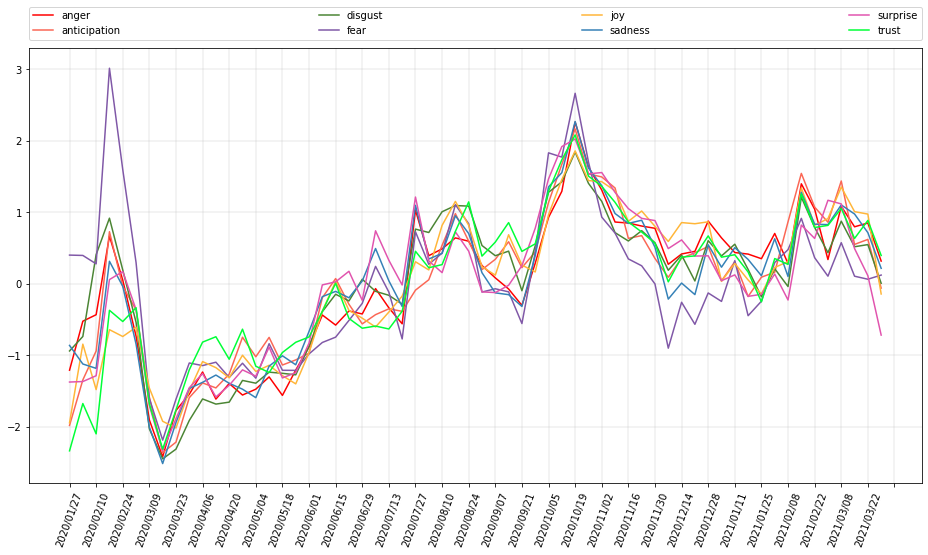
\includegraphics[scale=.3]{assets/img/it_emotions_normalized.png}
    	\caption{Emotions expressed in Italian tweets per week, normalized w.r.t. the displayed period.}
    	\label{fig:it_emotion_weekly_norm}
    \end{figure}

\end{frame}

\subsection{Peaks}
\begin{frame}{Most used Italian words 2020/02/17 - 23}
	
	The result of a peak analysis is showed below: notice that the same word in the lexicon has been associated with different emotions. In fact, it is very difficult to understand the sentiment that the user wanted to convey without knowing the context.
	
	\begin{figure}[h]
    	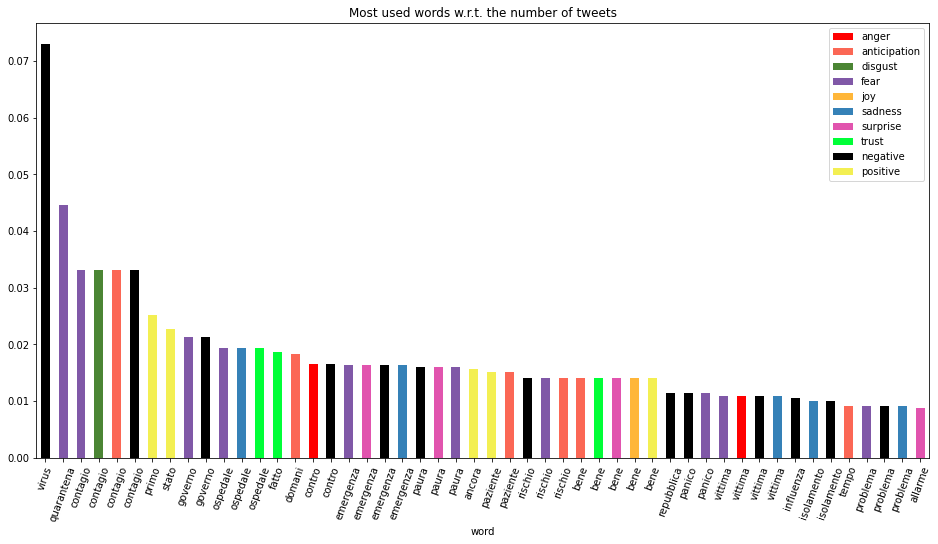
\includegraphics[scale=.3]{assets/img/it_2020_02_17_most_used_words.png}
    	\caption{Most used Italian words from 2020/02/17 to 2020/02/23}
    	\label{fig:it_2020_02_17_most_used_words}
    \end{figure}
	
\end{frame}

\begin{frame}{Most used Italian words 2020/02/17 - 23 (subplot)}
	
	\begin{figure}[h]
    	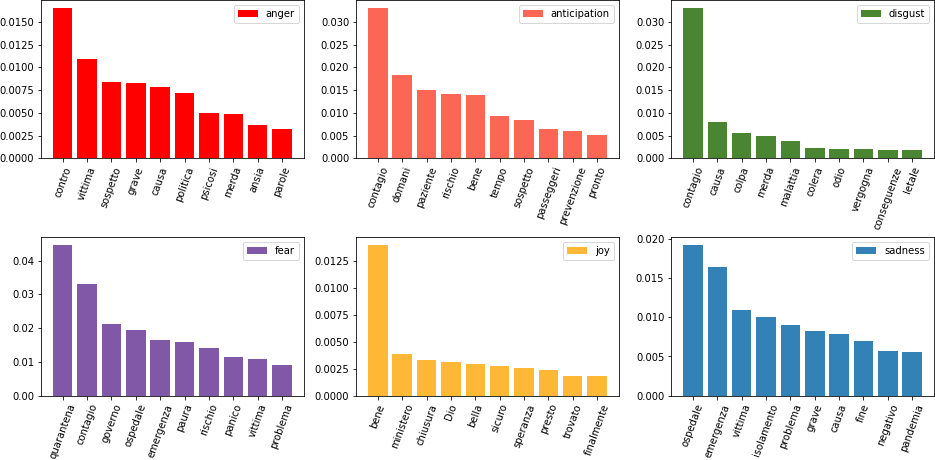
\includegraphics[scale=.32]{assets/img/it_2020_02_17_most_used_words_subplots_1.png}
    	\caption{Most used Italian words from 2020/02/17 to 2020/02/23 per emotion \#1}
    	\label{fig:it_2020_02_17_most_used_words_subplots_1}
    \end{figure}
	
\end{frame}

\begin{frame}{Most used Italian words 2020/02/17 - 23 (subplot)}
	
	\begin{figure}[h]
    	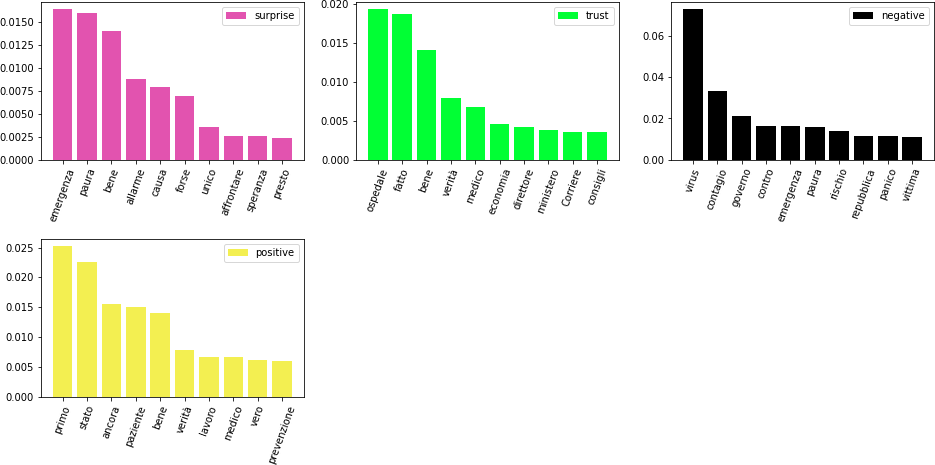
\includegraphics[scale=.32]{assets/img/it_2020_02_17_most_used_words_subplots_2.png}
    	\caption{Most used Italian words from 2020/02/17 to 2020/02/23 per emotion \#2}
    	\label{fig:it_2020_02_17_most_used_words_subplots_2}
    \end{figure}
	
\end{frame}
\section{Sentiment analysis over time - by gender}
\subsection{m3inference}
\begin{frame}[fragile]{Users inference}

	To infer data about the users, we used m3inference\autocite{wang2019demographic}, a \textbf{deep learning system for demographic inference} (gender, age, and person/organization) available on Python.
	
	m3inference bases its results on the analysis of the user's
	
	\begin{itemize}
	    \item description
	    \item name 
	    \item screen name
	    \item profile image
	\end{itemize}
	
	\begin{block}{m3inference prediction}
	    \begin{lstlisting}[language=json]
{
    "gender": {"male": 0.8758, "female": 0.1242}, 
    "age": {"<=18": 0.0053, "19-29": 0.0363, "30-39": 0.9239, ">=40": 0.0346}, 
    "org": {"non-org": 0.9965, "is-org": 0.0035}
}
	    \end{lstlisting}
	\end{block}
	
\end{frame}

\begin{frame}{Personal contribution}

	During the project I encountered several errors while using m3inference, for this reason I decided to open a Pull Request on GitHub\footnote{Pull request: \href{https://github.com/euagendas/m3inference/pull/20}{fix urllib errors while trying to fetch a profile image from twitter \#20}} to contribute to the project.
	
	\begin{figure}
	    \centering
	    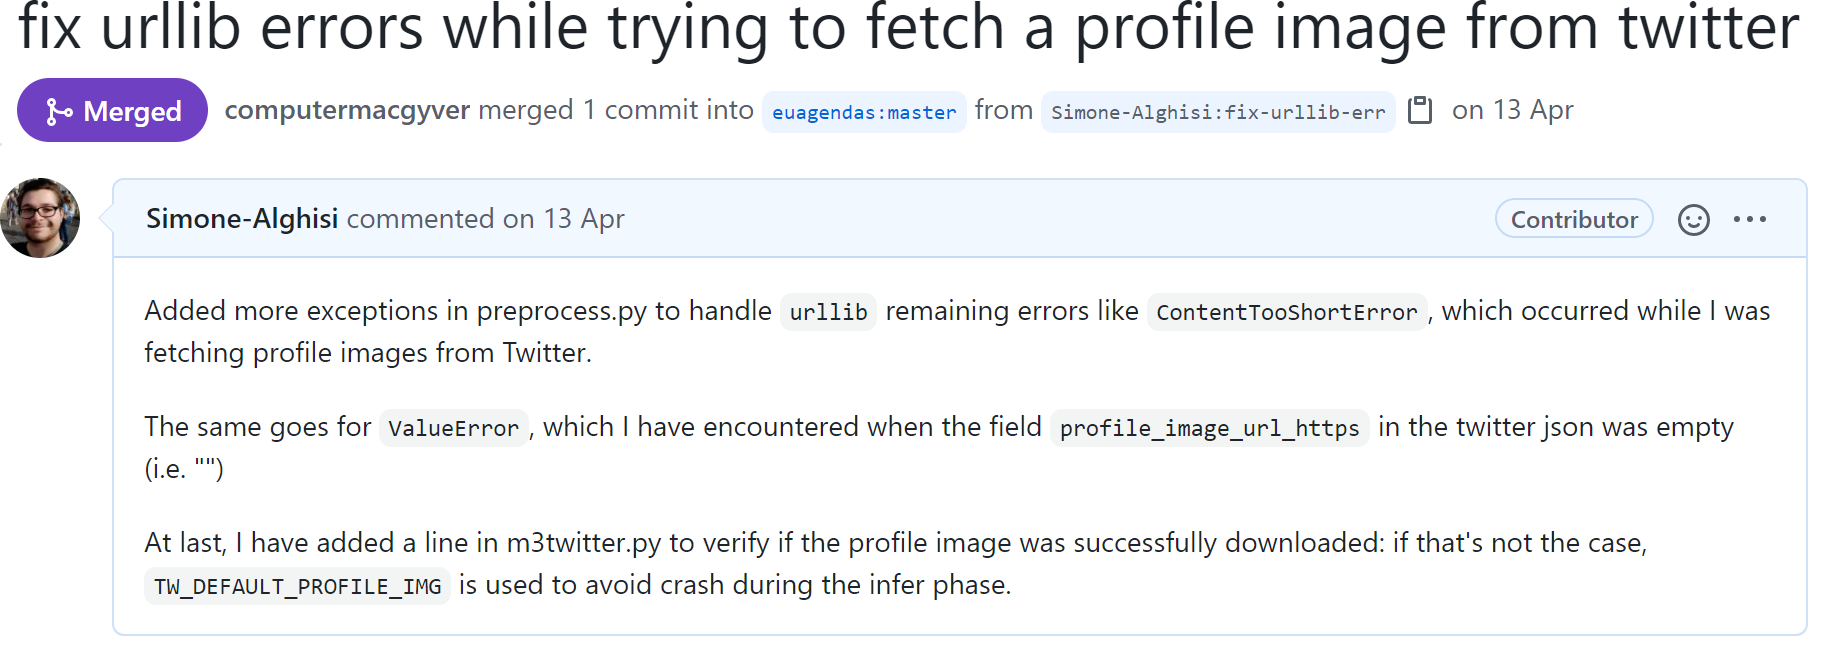
\includegraphics[scale=0.165]{assets/img/pull_request.png}
	\end{figure}
	
	The version of m3inference on the packet manager was updated when the same issue was notified by another user\footnote{issue: \href{https://github.com/euagendas/m3inference/issues/21}{Error fetching images will fail the infer method \#21}}.
	
\end{frame}

\begin{frame}{Prediction confidence}

    \begin{definition}
        A user \(u\) belongs to the category \(c \in C\) iif their prediction confidence \(pc\) is greater or equal than 0.95, i.e.
	    \[u \in c \Longleftrightarrow pc(u) \geq 0.95\]
	\end{definition}
	
	In particular, the following methodology was applied
	
	\begin{itemize}
	    \item we first check if the user's account belongs to an organization
	    \item then, if the user is male (or female)
	    \item finally, if none of the previous constraints were satisfied, we do not consider this user
	\end{itemize}
	
\end{frame}

\subsection{Results per week}

\begin{frame}{Italian tweets per week with user categories}

	In the graphics below it is possible to observe the emotions course divided by week and also per category. The gray line shows the general course of the emotion (i.e. without considering the division per category) 
	
	\begin{figure}[h]
    	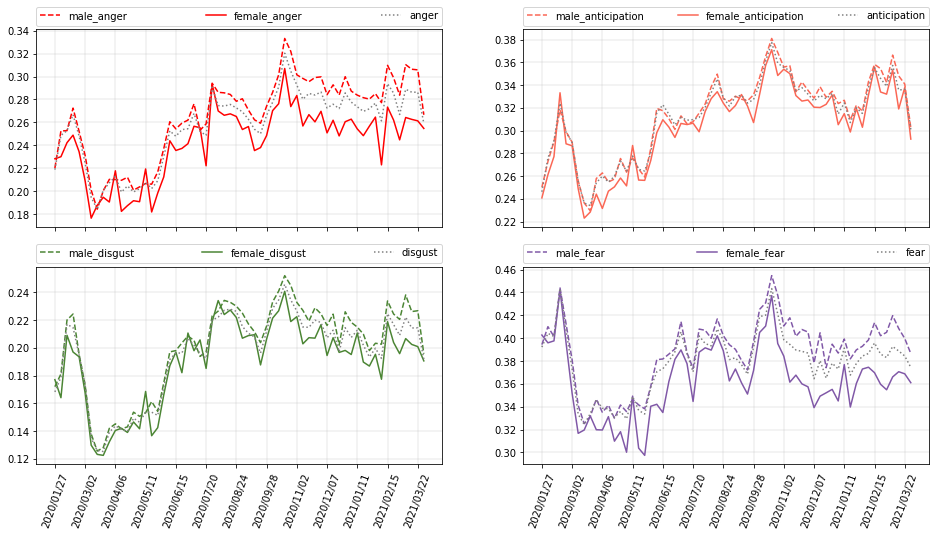
\includegraphics[scale=.30]{assets/img/it_emotions_per_category_wrt_total_subplots_1.png}
    	\caption{Emotions expressed in Italian tweets per week and category \#1}
    	\label{fig:it_emotion_weekly_per_category_subplot_1}
    \end{figure}
	
\end{frame}

\begin{frame}{Italian tweets per week with user categories} 
	
	\begin{figure}[h]
    	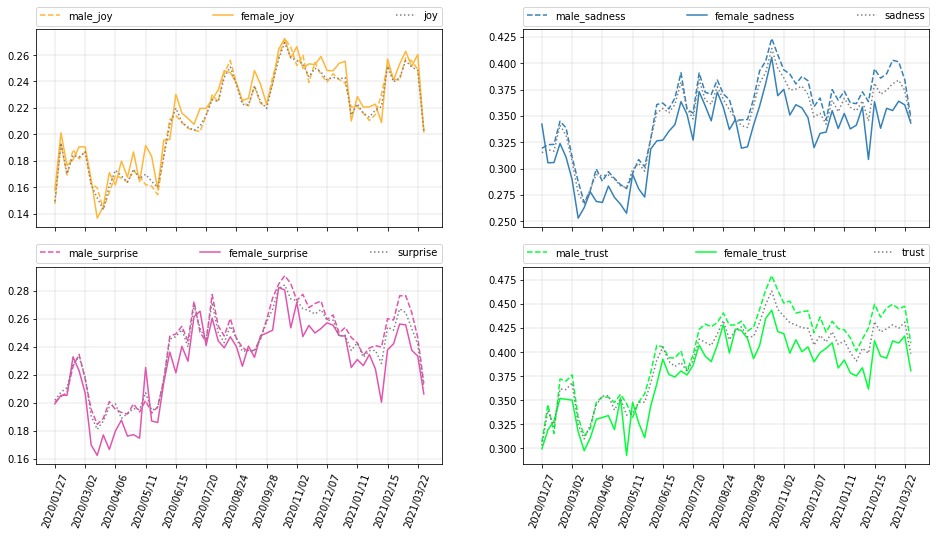
\includegraphics[scale=.30]{assets/img/it_emotions_per_category_wrt_total_subplots_2.png}
    	\caption{Emotions expressed in Italian tweets per week and category \#2}
    	\label{fig:it_emotion_weekly_per_category_subplot_2}
    \end{figure}
	
\end{frame}

\subsection{Data normalization}

\begin{frame}{Data normalization (categories)}
	
	Instead, \cref{fig:it_emotion_weekly_per_category_proportion_subplot_1} and \cref{fig:it_emotion_weekly_per_category_proportion_subplot_2} below, are meant to show whether a certain category \(c \in C\) expressed at time \(t\) more (or less) emotion \(e\) (e.g. sadness, anger) w.r.t the mean value for emotion \(e\) in the period of time \([0, T]\), regardless of the category.
	
	\begin{definition}
	    Given \(f_{e, c}(t)\), i.e. the proportion of users belonging to category \(c \in C\) that expressed emotion \(e\) at time \(t\), and the period of time \([0,T]\),
	    
	    \[v_{e, c}(t) = \frac{f_{e, c}(t) - \mu_{[0,T]}(f_e)}{\mu_{[0,T]}(f_e)}\]
	    
	    \[\text{where } \mu_{[0,T]}(f_e) = \frac{1}{\mid T \mid} \sum_{t =0}^{T} f_e(t) = \frac{1}{\mid T \mid} \sum_{t =0}^{T} \sum_{c \in C} f_{e, c}(t)\] 
	\end{definition}
	
\end{frame}

\begin{frame}{Italian tweets per week with user categories}
	
	\begin{figure}[h]
    	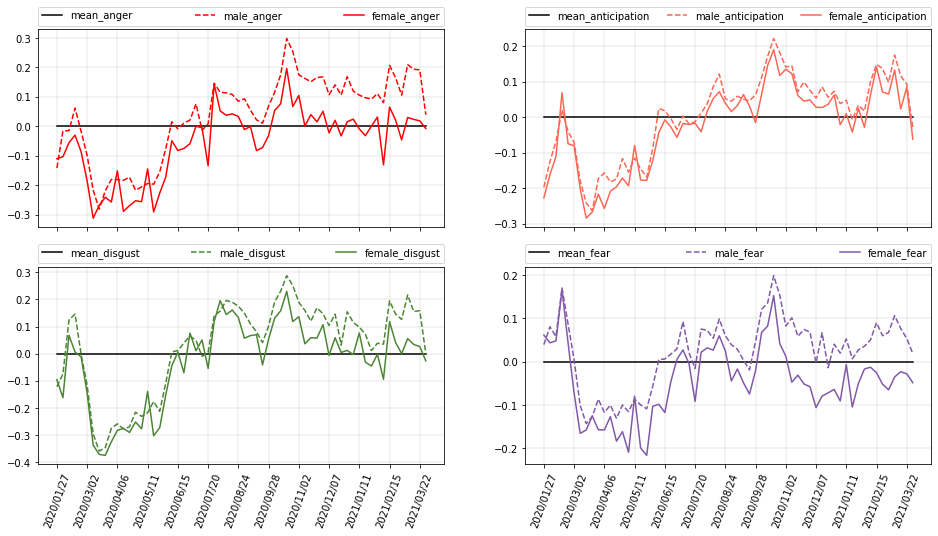
\includegraphics[scale=.30]{assets/img/it_emotions_per_category_wrt_total_proportion_subplots_1.png}
    	\caption{Value of the emotions per category w.r.t the average value among all users \#1}
    	\label{fig:it_emotion_weekly_per_category_proportion_subplot_1}
    \end{figure}
	
\end{frame}

\begin{frame}{Italian tweets per week with user categories} 
	
	\begin{figure}[h]
    	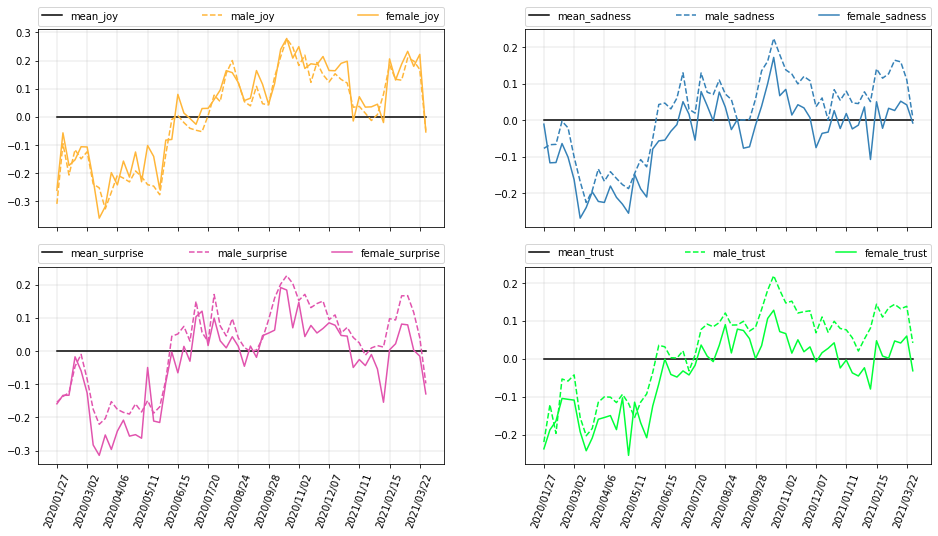
\includegraphics[scale=.30]{assets/img/it_emotions_per_category_wrt_total_proportion_subplots_2.png}
    	\caption{Value of the emotions per category w.r.t average value among all users \#2}
    	\label{fig:it_emotion_weekly_per_category_proportion_subplot_2}
    \end{figure}
	
\end{frame}

\section{Sentiment analysis over time - by region}
\begin{frame}{Users locations}
    
    Users on Twitter can specify their location so, for the third sentiment analysis, we thought about \textbf{analyzing the emotions of the users from a specific location} (e.g. state, country, \ldots).
    
    Unfortunately, Twitter does not provide any format or restriction for the location, so
    \begin{itemize}
        \item not all the users inserted a location
        \item some locations could be fake or misspelled
        \item the same location could be specified with a different syntax
    \end{itemize}
    
\end{frame}

\subsection{OpenStreetMap}
\begin{frame}{Geocoding}

    We linked the users to a specific place through \textbf{address geocoding}. Address geocoding is the process of taking a text-based description of a location and returning its geographic coordinates.
    
    \begin{figure}
        \centering
        
\includegraphics[scale=.25]{assets/img/Openstreetmap_logo.pdf}
        \caption{OSM Logo}
        \label{fig:osm_logo}
    \end{figure}
    
    For this task, we decided to use the data made available by \textbf{OpenStreetMap (OSM)}\autocite{OpenStreetMap}, a collaborative project to create a free editable map of the world.
    
\end{frame}

\begin{frame}[fragile]{Request results}

    In particular, given a location we used
    
    \begin{itemize}
        \item \textbf{geopy}\footnote{Python client for several geocoding web services} to contact the Nominatim public API 
        \item \textbf{Nominatim}\footnote{tool to search through OSM data by name and address} to get the coordinates and the address
    \end{itemize}
    
    \begin{block}{Result obtained given "Milano" as location}
    	\begin{lstlisting}[language=json]
{
    "place_id": 317098601, 
    "licence": "Data \u00a9 OpenStreetMap contributors, ODbL 1.0. https://osm.org/copyright",
    "boundingbox": ["45.3867381", "45.5358482", "9.0408867", "9.2781103"], 
    "lat": "45.4668", 
    "lon": "9.1905", 
    "display_name": "Milano, Lombardia, Italia",
    "address": {
        "city": "Milano", 
        "county": "Milano",
        "state": "Lombardia", 
        "country": "Italia", 
        "country_code": "it"
    }
}
        \end{lstlisting}
	\end{block}
    
\end{frame}

\subsection{Geocode results}

\begin{frame}{Italian users distribution in Italy}

    After assigning to each user location its corresponding state, the following data were available:
    
    \begin{figure}
        \centering
        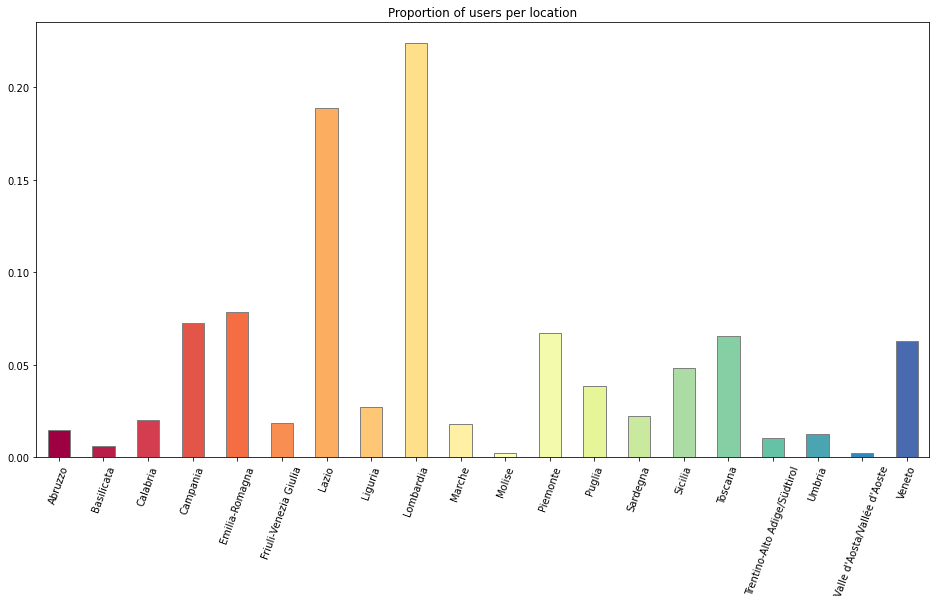
\includegraphics[scale=0.3]{assets/img/it_user_distribution.png}
        \caption{Italian users distribution in Italy per state}
        \label{fig:it_user_distribution}
    \end{figure}
    
\end{frame}

\subsection{Results per week}

\begin{frame}{Italian tweets expressing anger per week and state}
    
    \begin{figure}
        \centering
        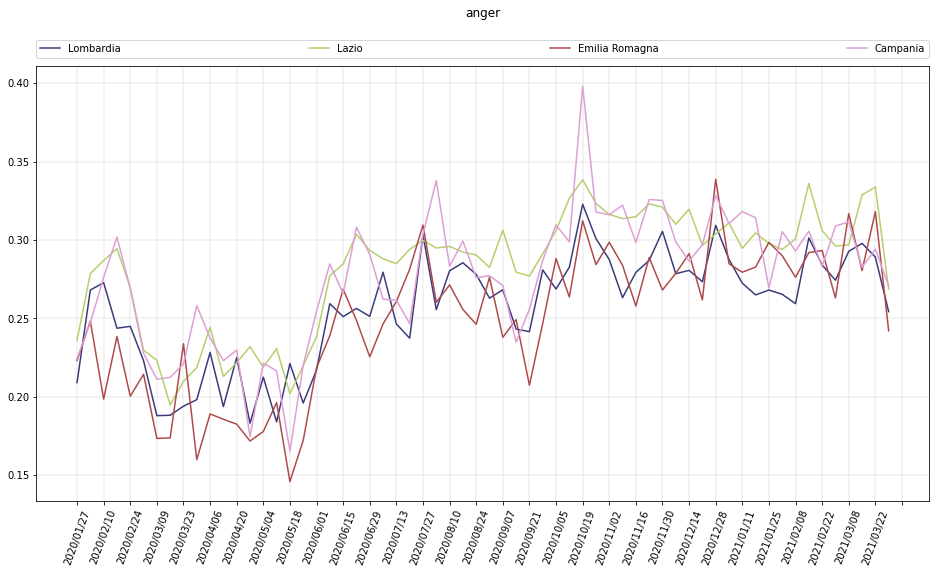
\includegraphics[scale=0.3]{assets/img/it_states_anger.png}
        \caption{Italian tweets expressing anger per week from Lombardia, Lazio, Emilia Romagna and Campania}
        \label{fig:it_states_anger}
    \end{figure}
    
\end{frame}

\begin{frame}{Italian tweets expressing joy per week and state}
    
    \begin{figure}
        \centering
        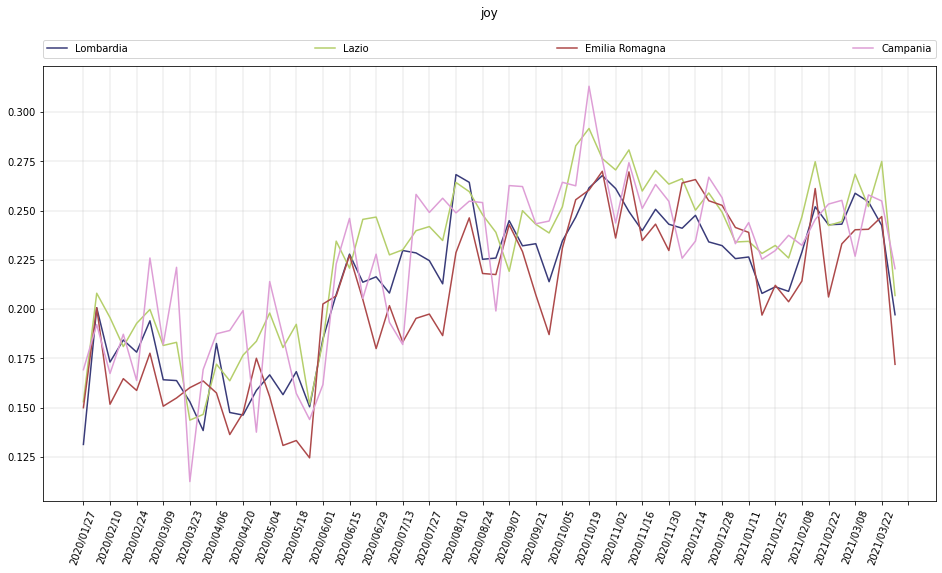
\includegraphics[scale=0.3]{assets/img/it_states_joy.png}
        \caption{Italian tweets expressing joy per week from Lombardia, Lazio, Emilia Romagna and Campania}
        \label{fig:it_states_joy}
    \end{figure}
    
\end{frame}

\begin{frame}{Tweets from Campania expressing anger per week}
    
    \begin{figure}
        \centering
        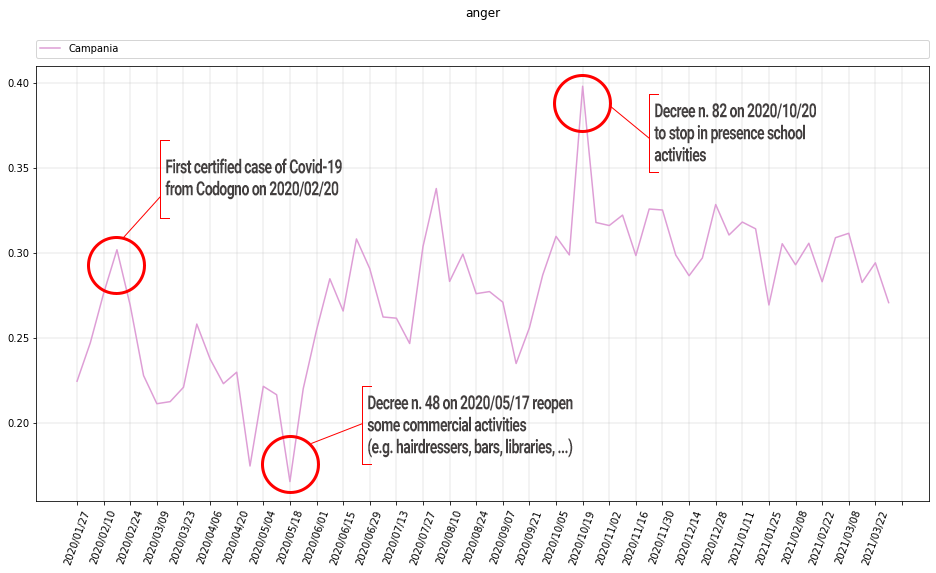
\includegraphics[scale=0.3]{assets/img/it_Campania_anger_with_events.png}
        \caption{Italian tweets from Campania expressing anger per week}
        \label{fig:it_Campania_anger}
    \end{figure}
    
\end{frame}

\begin{frame}{Tweets from Campania expressing joy per week}
    
    \begin{figure}
        \centering
        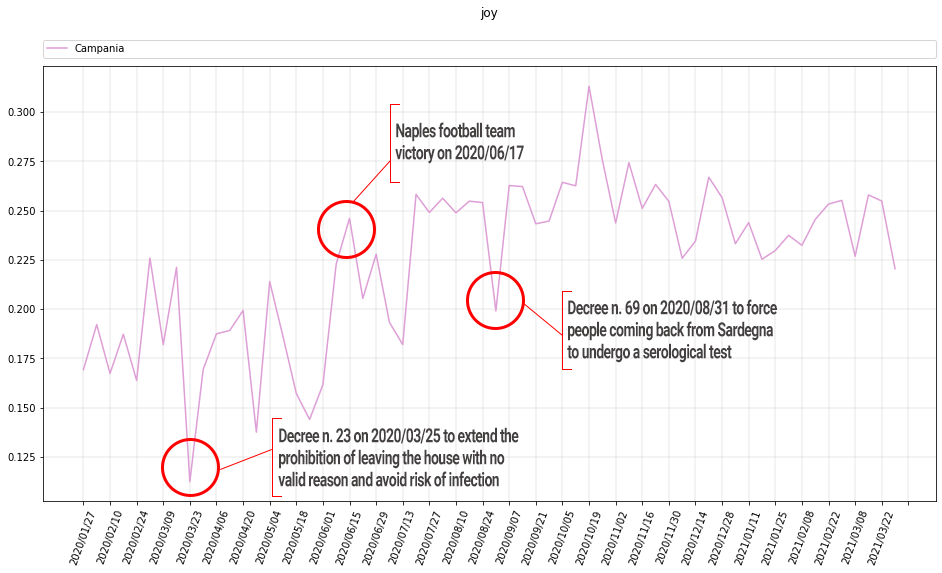
\includegraphics[scale=0.3]{assets/img/it_Campania_joy_with_events.png}
        \caption{Italian tweets from Campania expressing joy per week}
        \label{fig:it_Campania_joy}
    \end{figure}
    
\end{frame}

\section{Conclusions}

\begin{frame}{Final comments}
    
    During the project we were able to understand users' emotion in different ways:
    
    \begin{itemize}
        \item \textbf{categories analysis} showed that women in Italian tweets seems to express more joy through the whole period, and this make sense if we consider the fact that men expressed more negative emotions (e.g. anger, sadness)
        \item \textbf{locations analysis} was very useful to link certain emotional peaks to real world events
    \end{itemize}
    
    I was only able to scratch the surface of this research field and this impressive amount of data from Twitter, but I hope that my contribution could be a good starting point for further studies. 
    
\end{frame}

\section{Tools used}

\begin{frame}{Tools and Libraries used}

    \begin{itemize}
        \item Python, as main programming language to write the code for the project
        \item Pandas, to perform small operation on the datasets
        \item Matplotlib and Plotly, for data visualization
        \item Twarc, to retrieve (hydrate) tweets from Twitter using TweetIDs
        \item m3inference, a deep learning system for demographic inference (gender, age, and person/organization)
        \item geopy and Nominatim, to geocode the locations of the users
        \item NRC Word-Emotion Association Lexicon (aka EmoLex), to perform sentiment analysis on the tweets of the users
    \end{itemize}
    
\end{frame}

\section{Bibliography}

\begin{frame}[allowframebreaks]
        \frametitle{References}
        \printbibliography
\end{frame}

\end{document}
